\documentclass[]{ctexbook}
\usepackage{lmodern}
\usepackage{amssymb,amsmath}
\usepackage{ifxetex,ifluatex}
\usepackage{fixltx2e} % provides \textsubscript
\ifnum 0\ifxetex 1\fi\ifluatex 1\fi=0 % if pdftex
  \usepackage[T1]{fontenc}
  \usepackage[utf8]{inputenc}
\else % if luatex or xelatex
  \ifxetex
    \usepackage{xltxtra,xunicode}
  \else
    \usepackage{fontspec}
  \fi
  \defaultfontfeatures{Ligatures=TeX,Scale=MatchLowercase}
\fi
% use upquote if available, for straight quotes in verbatim environments
\IfFileExists{upquote.sty}{\usepackage{upquote}}{}
% use microtype if available
\IfFileExists{microtype.sty}{%
\usepackage{microtype}
\UseMicrotypeSet[protrusion]{basicmath} % disable protrusion for tt fonts
}{}
\usepackage[b5paper,tmargin=2.5cm,bmargin=2.5cm,lmargin=3.5cm,rmargin=2.5cm]{geometry}
\usepackage[unicode=true]{hyperref}
\PassOptionsToPackage{usenames,dvipsnames}{color} % color is loaded by hyperref
\hypersetup{
            pdftitle={R中的统计模拟},
            pdfauthor={wang},
            colorlinks=true,
            linkcolor=Maroon,
            citecolor=Blue,
            urlcolor=Blue,
            breaklinks=true}
\urlstyle{same}  % don't use monospace font for urls
\usepackage{natbib}
\bibliographystyle{apalike}
\usepackage{color}
\usepackage{fancyvrb}
\newcommand{\VerbBar}{|}
\newcommand{\VERB}{\Verb[commandchars=\\\{\}]}
\DefineVerbatimEnvironment{Highlighting}{Verbatim}{commandchars=\\\{\}}
% Add ',fontsize=\small' for more characters per line
\usepackage{framed}
\definecolor{shadecolor}{RGB}{248,248,248}
\newenvironment{Shaded}{\begin{snugshade}}{\end{snugshade}}
\newcommand{\AlertTok}[1]{\textcolor[rgb]{0.94,0.16,0.16}{#1}}
\newcommand{\AnnotationTok}[1]{\textcolor[rgb]{0.56,0.35,0.01}{\textbf{\textit{#1}}}}
\newcommand{\AttributeTok}[1]{\textcolor[rgb]{0.77,0.63,0.00}{#1}}
\newcommand{\BaseNTok}[1]{\textcolor[rgb]{0.00,0.00,0.81}{#1}}
\newcommand{\BuiltInTok}[1]{#1}
\newcommand{\CharTok}[1]{\textcolor[rgb]{0.31,0.60,0.02}{#1}}
\newcommand{\CommentTok}[1]{\textcolor[rgb]{0.56,0.35,0.01}{\textit{#1}}}
\newcommand{\CommentVarTok}[1]{\textcolor[rgb]{0.56,0.35,0.01}{\textbf{\textit{#1}}}}
\newcommand{\ConstantTok}[1]{\textcolor[rgb]{0.00,0.00,0.00}{#1}}
\newcommand{\ControlFlowTok}[1]{\textcolor[rgb]{0.13,0.29,0.53}{\textbf{#1}}}
\newcommand{\DataTypeTok}[1]{\textcolor[rgb]{0.13,0.29,0.53}{#1}}
\newcommand{\DecValTok}[1]{\textcolor[rgb]{0.00,0.00,0.81}{#1}}
\newcommand{\DocumentationTok}[1]{\textcolor[rgb]{0.56,0.35,0.01}{\textbf{\textit{#1}}}}
\newcommand{\ErrorTok}[1]{\textcolor[rgb]{0.64,0.00,0.00}{\textbf{#1}}}
\newcommand{\ExtensionTok}[1]{#1}
\newcommand{\FloatTok}[1]{\textcolor[rgb]{0.00,0.00,0.81}{#1}}
\newcommand{\FunctionTok}[1]{\textcolor[rgb]{0.00,0.00,0.00}{#1}}
\newcommand{\ImportTok}[1]{#1}
\newcommand{\InformationTok}[1]{\textcolor[rgb]{0.56,0.35,0.01}{\textbf{\textit{#1}}}}
\newcommand{\KeywordTok}[1]{\textcolor[rgb]{0.13,0.29,0.53}{\textbf{#1}}}
\newcommand{\NormalTok}[1]{#1}
\newcommand{\OperatorTok}[1]{\textcolor[rgb]{0.81,0.36,0.00}{\textbf{#1}}}
\newcommand{\OtherTok}[1]{\textcolor[rgb]{0.56,0.35,0.01}{#1}}
\newcommand{\PreprocessorTok}[1]{\textcolor[rgb]{0.56,0.35,0.01}{\textit{#1}}}
\newcommand{\RegionMarkerTok}[1]{#1}
\newcommand{\SpecialCharTok}[1]{\textcolor[rgb]{0.00,0.00,0.00}{#1}}
\newcommand{\SpecialStringTok}[1]{\textcolor[rgb]{0.31,0.60,0.02}{#1}}
\newcommand{\StringTok}[1]{\textcolor[rgb]{0.31,0.60,0.02}{#1}}
\newcommand{\VariableTok}[1]{\textcolor[rgb]{0.00,0.00,0.00}{#1}}
\newcommand{\VerbatimStringTok}[1]{\textcolor[rgb]{0.31,0.60,0.02}{#1}}
\newcommand{\WarningTok}[1]{\textcolor[rgb]{0.56,0.35,0.01}{\textbf{\textit{#1}}}}
\usepackage{longtable,booktabs}
% Fix footnotes in tables (requires footnote package)
\IfFileExists{footnote.sty}{\usepackage{footnote}\makesavenoteenv{long table}}{}
\usepackage{graphicx,grffile}
\makeatletter
\def\maxwidth{\ifdim\Gin@nat@width>\linewidth\linewidth\else\Gin@nat@width\fi}
\def\maxheight{\ifdim\Gin@nat@height>\textheight\textheight\else\Gin@nat@height\fi}
\makeatother
% Scale images if necessary, so that they will not overflow the page
% margins by default, and it is still possible to overwrite the defaults
% using explicit options in \includegraphics[width, height, ...]{}
\setkeys{Gin}{width=\maxwidth,height=\maxheight,keepaspectratio}
\IfFileExists{parskip.sty}{%
\usepackage{parskip}
}{% else
\setlength{\parindent}{0pt}
\setlength{\parskip}{6pt plus 2pt minus 1pt}
}
\setlength{\emergencystretch}{3em}  % prevent overfull lines
\providecommand{\tightlist}{%
  \setlength{\itemsep}{0pt}\setlength{\parskip}{0pt}}
\setcounter{secnumdepth}{5}
% Redefines (sub)paragraphs to behave more like sections
\ifx\paragraph\undefined\else
\let\oldparagraph\paragraph
\renewcommand{\paragraph}[1]{\oldparagraph{#1}\mbox{}}
\fi
\ifx\subparagraph\undefined\else
\let\oldsubparagraph\subparagraph
\renewcommand{\subparagraph}[1]{\oldsubparagraph{#1}\mbox{}}
\fi

% set default figure placement to htbp
\makeatletter
\def\fps@figure{htbp}
\makeatother

\usepackage{booktabs}
\usepackage{longtable}

\usepackage{framed,color}
\definecolor{shadecolor}{RGB}{248,248,248}

\renewcommand{\textfraction}{0.05}
\renewcommand{\topfraction}{0.8}
\renewcommand{\bottomfraction}{0.8}
\renewcommand{\floatpagefraction}{0.75}

\let\oldhref\href
\renewcommand{\href}[2]{#2\footnote{\url{#1}}}

\makeatletter
\newenvironment{kframe}{%
\medskip{}
\setlength{\fboxsep}{.8em}
 \def\at@end@of@kframe{}%
 \ifinner\ifhmode%
  \def\at@end@of@kframe{\end{minipage}}%
  \begin{minipage}{\columnwidth}%
 \fi\fi%
 \def\FrameCommand##1{\hskip\@totalleftmargin \hskip-\fboxsep
 \colorbox{shadecolor}{##1}\hskip-\fboxsep
     % There is no \\@totalrightmargin, so:
     \hskip-\linewidth \hskip-\@totalleftmargin \hskip\columnwidth}%
 \MakeFramed {\advance\hsize-\width
   \@totalleftmargin\z@ \linewidth\hsize
   \@setminipage}}%
 {\par\unskip\endMakeFramed%
 \at@end@of@kframe}
\makeatother

\makeatletter
\@ifundefined{Shaded}{
}{\renewenvironment{Shaded}{\begin{kframe}}{\end{kframe}}}
\@ifpackageloaded{fancyvrb}{%
  % https://github.com/CTeX-org/ctex-kit/issues/331
  \RecustomVerbatimEnvironment{Highlighting}{Verbatim}{commandchars=\\\{\},formatcom=\xeCJKVerbAddon}%
}{}
\makeatother

\usepackage{makeidx}
\makeindex

\urlstyle{tt}

\usepackage{amsthm}
\makeatletter
\def\thm@space@setup{%
  \thm@preskip=8pt plus 2pt minus 4pt
  \thm@postskip=\thm@preskip
}
\makeatother

\frontmatter

\title{R中的统计模拟}
\author{wang}
\date{2019-08-05}

\begin{document}
\maketitle


\thispagestyle{empty}

\begin{center}
献给……

呃,爱谁谁吧
\end{center}

\setlength{\abovedisplayskip}{-5pt}
\setlength{\abovedisplayshortskip}{-5pt}

{
\setcounter{tocdepth}{2}
\tableofcontents
}
\listoftables
\listoffigures
\hypertarget{section}{%
\chapter*{前言}\label{section}}


关于R的基础语法,可以在网上或者书籍中学习.

\href{https://github.com/yanping/r-spring-camp/blob/master/1-introduction.md}{Github}

\href{https://www.w3cschool.cn/r/r_overview.html}{W3Cschool}

\href{https://adv-r.hadley.nz}{Advanced R}

这里只是总结一些统计模拟中遇到的问题,以及实用的技巧.

\hypertarget{section-1}{%
\section*{致谢}\label{section-1}}


这个页面的建立基于 \textbf{knitr}\index{knitr} \citep{xie2015}和 \textbf{bookdown}\index{bookdown} \citep{R-bookdown}。以下是我的 R 进程信息:

\begin{Shaded}
\begin{Highlighting}[]
\KeywordTok{sessionInfo}\NormalTok{()}
\end{Highlighting}
\end{Shaded}

\begin{verbatim}
## R version 3.6.0 (2019-04-26)
## Platform: x86_64-apple-darwin15.6.0 (64-bit)
## Running under: macOS Mojave 10.14.6
## 
## Matrix products: default
## BLAS:   /Library/Frameworks/R.framework/Versions/3.6/Resources/lib/libRblas.0.dylib
## LAPACK: /Library/Frameworks/R.framework/Versions/3.6/Resources/lib/libRlapack.dylib
## 
## locale:
## [1] en_US.UTF-8/en_US.UTF-8/en_US.UTF-8/C/en_US.UTF-8/en_US.UTF-8
## 
## attached base packages:
## [1] parallel  stats     graphics  grDevices utils    
## [6] datasets  methods   base     
## 
## other attached packages:
## [1] doParallel_1.0.14 iterators_1.0.10 
## [3] foreach_1.4.4     MASS_7.3-51.4    
## [5] quadprog_1.5-7   
## 
## loaded via a namespace (and not attached):
##  [1] beeswarm_0.2.3     tidyselect_0.2.5  
##  [3] xfun_0.7           Rook_1.1-1        
##  [5] purrr_0.3.2        colorspace_1.4-1  
##  [7] vctrs_0.2.0        htmltools_0.3.6   
##  [9] viridisLite_0.3.0  yaml_2.2.0        
## [11] XML_3.98-1.20      rlang_0.4.0       
## [13] pillar_1.4.2       glue_1.3.1        
## [15] RColorBrewer_1.1-2 plyr_1.8.4        
## [17] stringr_1.4.0      munsell_0.5.0     
## [19] gtable_0.3.0       visNetwork_2.0.7  
## [21] htmlwidgets_1.3    bench_1.0.2.9000  
## [23] codetools_0.2-16   evaluate_0.14     
## [25] knitr_1.23         vipor_0.4.5       
## [27] DiagrammeR_1.0.1   profmem_0.5.0     
## [29] highr_0.8          Rcpp_1.0.1        
## [31] xtable_1.8-4       readr_1.3.1       
## [33] backports_1.1.4    scales_1.0.0      
## [35] jsonlite_1.6       rgexf_0.15.3      
## [37] gridExtra_2.3      brew_1.0-6        
## [39] ggplot2_3.1.1      hms_0.5.0         
## [41] digest_0.6.19      stringi_1.4.3     
## [43] bookdown_0.11      dplyr_0.8.1       
## [45] grid_3.6.0         influenceR_0.1.0  
## [47] tools_3.6.0        magrittr_1.5      
## [49] lazyeval_0.2.2     tibble_2.1.3      
## [51] crayon_1.3.4       tidyr_0.8.3       
## [53] pkgconfig_2.0.2    zeallot_0.1.0     
## [55] downloader_0.4     ggbeeswarm_0.6.0  
## [57] assertthat_0.2.1   rmarkdown_1.13    
## [59] rstudioapi_0.10    viridis_0.5.1     
## [61] R6_2.4.0           igraph_1.2.4.1    
## [63] compiler_3.6.0
\end{verbatim}

\hypertarget{author}{%
\chapter*{作者简介}\label{author}}


统计学学生.

主要用R和tex.

\mainmatter

\hypertarget{section-2}{%
\chapter{常用函数及常见错误}\label{section-2}}

\hypertarget{section-3}{%
\section{产生数据}\label{section-3}}

在进行模拟时, 我们经常会需要生成数据. 这里以正态分布为例, 说明如 何产生数据. 在 R 中, 每种分布都会有以下 4 个函数:

\begin{itemize}
\tightlist
\item
  概率密度函数: dnorm(x, mean = 0, sd = 1, log = FALSE)
\item
  累计分布函数: pnorm(q, mean = 0, sd = 1, lower.tail = TRUE, log.p = FALSE)
\item
  分位数函数: qnorm(p, mean = 0, sd = 1, lower.tail = TRUE, log.p = FALSE)
\item
  随机数产生: rnorm(n, mean = 0, sd = 1):
\end{itemize}

其中前 3 个函数都支持向量输入, 即计算一组取值的概率密度、累计分布、 分位数. 最后一个函数常用来生成数据,n 即产生数据的个数. 如果需要生成 多维正态分布, 需要调用 MASS 包中的
*mvrnorm(n = 1, mu, Sigma, tol = 1e-6, empirical = FALSE, EISPACK = FALSE),
其中 Sigma 是指定的协方差矩阵.

\hypertarget{section-4}{%
\section{定义运算符}\label{section-4}}

空间模型 (SAR) 中, 会出现对角块矩阵 \[ \mathbf{W}=\left(\begin{array}{cccc}{\mathbf{M}} & {} & {} & {} \\ {} & {\mathbf{M}} & {} & {} \\ {} & {} & {\ddots} & {} \\ {} & {} & {} & {\mathbf{M}}\end{array}\right) \]

M 作为权重矩阵, 这种形式的矩阵可以利用克罗内克积 (Kronecker product, 符号为\(\otimes\)) 在 R 中很方便的产生,命令是\%x\%.
可以写成\[\mathbf{W} = \mathbf{I} \otimes \mathbf{M}.\]

\begin{Shaded}
\begin{Highlighting}[]
\KeywordTok{diag}\NormalTok{(}\DecValTok{3}\NormalTok{)}\OperatorTok\KeywordTok{matrix}\NormalTok{(}\DecValTok{1}\OperatorTok{:}\DecValTok{6}\NormalTok{,}\DecValTok{2}\NormalTok{,}\DecValTok{3}\NormalTok{)}
\end{Highlighting}
\end{Shaded}

\begin{verbatim}
##      [,1] [,2] [,3] [,4] [,5] [,6] [,7] [,8] [,9]
## [1,]    1    3    5    0    0    0    0    0    0
## [2,]    2    4    6    0    0    0    0    0    0
## [3,]    0    0    0    1    3    5    0    0    0
## [4,]    0    0    0    2    4    6    0    0    0
## [5,]    0    0    0    0    0    0    1    3    5
## [6,]    0    0    0    0    0    0    2    4    6
\end{verbatim}

这是借助自定义运算符实现的.自定义运算符是一种特殊的函数,当参数只有两个变量时,可以进行定义.用法如下:

\begin{Shaded}
\begin{Highlighting}[]
\StringTok{'%myop%'}\NormalTok{<-}\ControlFlowTok{function}\NormalTok{(a,b)\{a}\OperatorTok{^}\NormalTok{b}\OperatorTok{+}\NormalTok{b}\OperatorTok{^}\NormalTok{a\}}
\DecValTok{2}\OperatorTok\DecValTok{3}
\end{Highlighting}
\end{Shaded}

\begin{verbatim}
## [1] 17
\end{verbatim}

利用自定义运算符,可以实现很方便的功能.R中矩阵乘法(\%*\%)、Kronecker乘积(\%x\%)都是这样实现的.另外还有整除(\%/\%)和取余(\%\%)

\begin{Shaded}
\begin{Highlighting}[]
\DecValTok{9}\OperatorTok\DecValTok{4}
\end{Highlighting}
\end{Shaded}

\begin{verbatim}
## [1] 2
\end{verbatim}

\begin{Shaded}
\begin{Highlighting}[]
\DecValTok{13}\OperatorTok\DecValTok{3}
\end{Highlighting}
\end{Shaded}

\begin{verbatim}
## [1] 1
\end{verbatim}

\hypertarget{section-5}{%
\section{自动纠错}\label{section-5}}

当我们输入的命令不规范时,R会自动纠正,以保证程序正常运行.

比如看下面的例子:

\begin{Shaded}
\begin{Highlighting}[]
\DecValTok{1}\OperatorTok{:}\DecValTok{4} \OperatorTok{-}\StringTok{ }\DecValTok{1}\OperatorTok{:}\DecValTok{2}
\end{Highlighting}
\end{Shaded}

\begin{verbatim}
## [1] 0 0 2 2
\end{verbatim}

\begin{Shaded}
\begin{Highlighting}[]
\DecValTok{1}\OperatorTok{:}\DecValTok{5-1}\OperatorTok{:}\DecValTok{2}
\end{Highlighting}
\end{Shaded}

\begin{verbatim}
## Warning in 1:5 - 1:2: longer object length is not a
## multiple of shorter object length
\end{verbatim}

\begin{verbatim}
## [1] 0 0 2 2 4
\end{verbatim}

当运算的向量长度不一致时,R会自动重复短的向量,使之长度与另外的向量长度相同进行运算.但是当长度是整数倍当时候,不会有任何提示.

再看下面当例子:

\begin{Shaded}
\begin{Highlighting}[]
\KeywordTok{matrix}\NormalTok{(}\DecValTok{1}\OperatorTok{:}\DecValTok{9}\NormalTok{,}\DecValTok{3}\NormalTok{,}\DecValTok{3}\NormalTok{)}\OperatorTok{*}\NormalTok{(}\DecValTok{1}\OperatorTok{:}\DecValTok{3}\NormalTok{)}
\end{Highlighting}
\end{Shaded}

\begin{verbatim}
##      [,1] [,2] [,3]
## [1,]    1    4    7
## [2,]    4   10   16
## [3,]    9   18   27
\end{verbatim}

本来想计算矩阵与向量的乘积,但是错误使用了*,
未使用矩阵乘法\%*\%,R也可以计算返回一个矩阵,不会有warning.

当条件为向量是,只会判断第一个值:

\begin{Shaded}
\begin{Highlighting}[]
\ControlFlowTok{if}\NormalTok{( }\DecValTok{1} \OperatorTok{<=}\StringTok{ }\DecValTok{1}\OperatorTok{:}\DecValTok{3}\NormalTok{) }\KeywordTok{print}\NormalTok{(}\StringTok{"真"}\NormalTok{)  }\ControlFlowTok{else} \KeywordTok{print}\NormalTok{(}\StringTok{"假"}\NormalTok{)}
\end{Highlighting}
\end{Shaded}

\begin{verbatim}
## Warning in if (1 <= 1:3) print("真") else print("假"):
## the condition has length > 1 and only the first element
## will be used
\end{verbatim}

\begin{verbatim}
## [1] "真"
\end{verbatim}

如果条件为向量,应该使用all或者any函数:

\begin{Shaded}
\begin{Highlighting}[]
\KeywordTok{all}\NormalTok{(}\DecValTok{1} \OperatorTok{<=}\StringTok{ }\DecValTok{1}\OperatorTok{:}\DecValTok{3}\NormalTok{)}
\end{Highlighting}
\end{Shaded}

\begin{verbatim}
## [1] TRUE
\end{verbatim}

\begin{Shaded}
\begin{Highlighting}[]
\KeywordTok{all}\NormalTok{(}\DecValTok{2} \OperatorTok{<=}\StringTok{ }\DecValTok{1}\OperatorTok{:}\DecValTok{3}\NormalTok{)}
\end{Highlighting}
\end{Shaded}

\begin{verbatim}
## [1] FALSE
\end{verbatim}

所有都真的时候返回TRUE.

\begin{Shaded}
\begin{Highlighting}[]
\KeywordTok{any}\NormalTok{(}\DecValTok{4} \OperatorTok{<=}\StringTok{ }\DecValTok{1}\OperatorTok{:}\DecValTok{3}\NormalTok{)}
\end{Highlighting}
\end{Shaded}

\begin{verbatim}
## [1] FALSE
\end{verbatim}

\begin{Shaded}
\begin{Highlighting}[]
\KeywordTok{any}\NormalTok{(}\DecValTok{2} \OperatorTok{<=}\StringTok{ }\DecValTok{1}\OperatorTok{:}\DecValTok{3}\NormalTok{)}
\end{Highlighting}
\end{Shaded}

\begin{verbatim}
## [1] TRUE
\end{verbatim}

只要有一个为真就返回TRUE.

\hypertarget{predict}{%
\section{predict函数}\label{predict}}

当我们拟合好一个模型时,下一步要做的就是评价模型好坏或者对新数据预测.这都需要将新的输入值带入模型中计算,得到预测值.区别只是有没有真值对比.对于简单模型,我们当然可以直接提取系数,自己计算预测值,但是当模型复杂时(比如时间序列模型),就不太容易操作.

R借助泛型函数\footnote{程序在 \href{\%22code/Rcpp-demo.cpp\%22}{这里} 查看,其中最后被/***R */夹住的部分是R程序,每次加载后会自动执行,方便调试.},编写模型都会提供summary、predict、plot等函数方便调用.但是在学习过程中发现经常会不小心错误使用,特此单独说明一下.下面以线性模型为例,先看正确的使用方法:

\begin{Shaded}
\begin{Highlighting}[]
\NormalTok{n=}\DecValTok{100}\NormalTok{;p=}\DecValTok{3}\NormalTok{;beta=}\KeywordTok{c}\NormalTok{(}\DecValTok{1}\NormalTok{,}\DecValTok{2}\NormalTok{,}\DecValTok{3}\NormalTok{);}
\NormalTok{X =}\StringTok{ }\KeywordTok{matrix}\NormalTok{(}\KeywordTok{rnorm}\NormalTok{(n}\OperatorTok{*}\NormalTok{p),n,p)}
\NormalTok{Y =}\StringTok{ }\NormalTok{X}\OperatorTok\NormalTok{beta }\OperatorTok{+}\StringTok{ }\KeywordTok{rnorm}\NormalTok{(n)}
\NormalTok{trainlist =}\StringTok{ }\KeywordTok{sample}\NormalTok{(}\DecValTok{1}\OperatorTok{:}\NormalTok{n,}\DecValTok{70}\NormalTok{)}
\NormalTok{regData =}\StringTok{ }\KeywordTok{data.frame}\NormalTok{(Y,X)}
\NormalTok{fitmodel =}\StringTok{ }\KeywordTok{lm}\NormalTok{(Y}\OperatorTok{~}\NormalTok{.,}\DataTypeTok{data=}\NormalTok{regData[trainlist,])}
\NormalTok{pe =}\StringTok{ }\KeywordTok{predict}\NormalTok{(fitmodel,}\DataTypeTok{newdata=}\NormalTok{regData[}\OperatorTok{-}\NormalTok{trainlist,])}
\KeywordTok{sum}\NormalTok{((pe}\OperatorTok{-}\NormalTok{regData[}\OperatorTok{-}\NormalTok{trainlist,}\DecValTok{1}\NormalTok{])}\OperatorTok{^}\DecValTok{2}\NormalTok{)}\OperatorTok{/}\KeywordTok{length}\NormalTok{(pe)}
\end{Highlighting}
\end{Shaded}

\begin{verbatim}
## [1] 1.02
\end{verbatim}

关键点:

\emph{所有数据存在一个数据框中
}通过下标控制训练集和测试集的数据

错误程序1:

\begin{Shaded}
\begin{Highlighting}[]
\NormalTok{n=}\DecValTok{100}\NormalTok{;p=}\DecValTok{3}\NormalTok{;beta=}\KeywordTok{c}\NormalTok{(}\DecValTok{1}\NormalTok{,}\DecValTok{2}\NormalTok{,}\DecValTok{3}\NormalTok{);}
\NormalTok{X =}\StringTok{ }\KeywordTok{matrix}\NormalTok{(}\KeywordTok{rnorm}\NormalTok{(n}\OperatorTok{*}\NormalTok{p),n,p)}
\NormalTok{Y =}\StringTok{ }\NormalTok{X}\OperatorTok\NormalTok{beta }\OperatorTok{+}\StringTok{ }\KeywordTok{rnorm}\NormalTok{(n)}
\NormalTok{fitmodel =}\StringTok{ }\KeywordTok{lm}\NormalTok{(Y}\OperatorTok{~}\NormalTok{X)}
\NormalTok{X2 =}\StringTok{ }\KeywordTok{matrix}\NormalTok{(}\KeywordTok{rnorm}\NormalTok{(n}\OperatorTok{*}\NormalTok{p),n,p)}
\NormalTok{Y2 =}\StringTok{ }\NormalTok{X2}\OperatorTok\NormalTok{beta }\OperatorTok{+}\StringTok{ }\KeywordTok{rnorm}\NormalTok{(n)}
\CommentTok{#predict(fitmodel,newdata = X2)数据格式错误,不能执行}
\NormalTok{pe =}\StringTok{ }\KeywordTok{predict}\NormalTok{(fitmodel,}\DataTypeTok{newdata =} \KeywordTok{data.frame}\NormalTok{(X2))}
\KeywordTok{sum}\NormalTok{((pe}\OperatorTok{-}\NormalTok{Y2)}\OperatorTok{^}\DecValTok{2}\NormalTok{)}\OperatorTok{/}\KeywordTok{length}\NormalTok{(Y2)}
\end{Highlighting}
\end{Shaded}

\begin{verbatim}
## [1] 21.74
\end{verbatim}

这个程序能明显看出问题,误差不应该这么大,但是程序没有任何warning.

错误程序2:

\begin{Shaded}
\begin{Highlighting}[]
\NormalTok{n=}\DecValTok{100}\NormalTok{;p=}\DecValTok{3}\NormalTok{;beta=}\KeywordTok{c}\NormalTok{(}\DecValTok{1}\NormalTok{,}\DecValTok{2}\NormalTok{,}\DecValTok{3}\NormalTok{);}
\NormalTok{X =}\StringTok{ }\KeywordTok{matrix}\NormalTok{(}\KeywordTok{rnorm}\NormalTok{(n}\OperatorTok{*}\NormalTok{p),n,p)}
\NormalTok{Y =}\StringTok{ }\NormalTok{X}\OperatorTok\NormalTok{beta }\OperatorTok{+}\StringTok{ }\KeywordTok{rnorm}\NormalTok{(n)}
\NormalTok{fitmodel =}\StringTok{ }\KeywordTok{lm}\NormalTok{(Y}\OperatorTok{~}\NormalTok{X)}
\NormalTok{X2 =}\StringTok{ }\KeywordTok{matrix}\NormalTok{(}\KeywordTok{rnorm}\NormalTok{(}\FloatTok{0.2}\OperatorTok{*}\NormalTok{n}\OperatorTok{*}\NormalTok{p),}\FloatTok{0.2}\OperatorTok{*}\NormalTok{n,p)}
\NormalTok{Y2 =}\StringTok{ }\NormalTok{X2}\OperatorTok\NormalTok{beta }\OperatorTok{+}\StringTok{ }\KeywordTok{rnorm}\NormalTok{(}\FloatTok{0.2}\OperatorTok{*}\NormalTok{n)}
\NormalTok{pe =}\StringTok{ }\KeywordTok{predict}\NormalTok{(fitmodel,}\DataTypeTok{newdata =} \KeywordTok{data.frame}\NormalTok{(X2))}
\end{Highlighting}
\end{Shaded}

\begin{verbatim}
## Warning: 'newdata' had 20 rows but variables found have
## 100 rows
\end{verbatim}

\begin{Shaded}
\begin{Highlighting}[]
\KeywordTok{length}\NormalTok{(pe)}
\end{Highlighting}
\end{Shaded}

\begin{verbatim}
## [1] 100
\end{verbatim}

修改测试数据的条数,使之与训练集数据量不同,可以发现warning.提示我们数据行数不一样.并且我们测试集合X2是20行,但是预测值pe返回的是100个值.问题在于predict函数使用不正确.

我们用all指令查看:

\begin{Shaded}
\begin{Highlighting}[]
\KeywordTok{all}\NormalTok{(}\KeywordTok{predict}\NormalTok{(fitmodel)}\OperatorTok{==}\KeywordTok{predict}\NormalTok{(fitmodel,}\DataTypeTok{newdata =} \KeywordTok{data.frame}\NormalTok{(X2)))}
\end{Highlighting}
\end{Shaded}

\begin{verbatim}
## Warning: 'newdata' had 20 rows but variables found have
## 100 rows
\end{verbatim}

\begin{verbatim}
## [1] TRUE
\end{verbatim}

就是说我们输入的参数没起到作用.

查看函数说明\footnote{垃圾回收(英语:Garbage Collection,缩写为GC),在计算机科学中是一种自动的存储器管理机制。当一个计算机上的动态存储器不再需要时,就应该予以释放,以让出存储器,这种存储器资源管理,称为垃圾回收。}

\begin{Shaded}
\begin{Highlighting}[]
\NormalTok{?predict.lm}
\end{Highlighting}
\end{Shaded}

\begin{longtable}[]{@{}ll@{}}
\toprule
\begin{minipage}[b]{0.13\columnwidth}\raggedright
参数\strut
\end{minipage} & \begin{minipage}[b]{0.81\columnwidth}\raggedright
说明\strut
\end{minipage}\tabularnewline
\midrule
\endhead
\begin{minipage}[t]{0.13\columnwidth}\raggedright
object\strut
\end{minipage} & \begin{minipage}[t]{0.81\columnwidth}\raggedright
Object of class inheriting from ``lm''\strut
\end{minipage}\tabularnewline
\begin{minipage}[t]{0.13\columnwidth}\raggedright
newdata\strut
\end{minipage} & \begin{minipage}[t]{0.81\columnwidth}\raggedright
An optional data frame in which to look for variables with which to predict. If omitted, the fitted values are used.\strut
\end{minipage}\tabularnewline
\begin{minipage}[t]{0.13\columnwidth}\raggedright
\ldots{}\strut
\end{minipage} & \begin{minipage}[t]{0.81\columnwidth}\raggedright
\strut
\end{minipage}\tabularnewline
\bottomrule
\end{longtable}

newdata不是必要的参数,当缺失时候会使用拟合模型的数据.
至于为什么输入的数据不能正确识别,因为名字不一样.R中参数的传递都是通过名字,我们在拟合lm时候,解释变量的名字叫`X',所以传入`X2'不会识别到.如果把`X2'改名成`X',即可正确预测\footnote{后续重新整理成Rmd格式.},比如看下面的程序:

\begin{Shaded}
\begin{Highlighting}[]
\NormalTok{n=}\DecValTok{100}\NormalTok{;p=}\DecValTok{3}\NormalTok{;beta=}\KeywordTok{c}\NormalTok{(}\DecValTok{1}\NormalTok{,}\DecValTok{2}\NormalTok{,}\DecValTok{3}\NormalTok{);}
\NormalTok{X =}\StringTok{ }\KeywordTok{matrix}\NormalTok{(}\KeywordTok{rnorm}\NormalTok{(n}\OperatorTok{*}\NormalTok{p),n,p)}
\NormalTok{Y =}\StringTok{ }\NormalTok{X}\OperatorTok\NormalTok{beta }\OperatorTok{+}\StringTok{ }\KeywordTok{rnorm}\NormalTok{(n)}
\NormalTok{fitmodel =}\StringTok{ }\KeywordTok{lm}\NormalTok{(Y}\OperatorTok{~}\NormalTok{X)}
\NormalTok{X =}\StringTok{ }\KeywordTok{matrix}\NormalTok{(}\KeywordTok{rnorm}\NormalTok{(}\FloatTok{0.2}\OperatorTok{*}\NormalTok{n}\OperatorTok{*}\NormalTok{p),}\FloatTok{0.2}\OperatorTok{*}\NormalTok{n,p)}
\NormalTok{Y2 =}\StringTok{ }\NormalTok{X}\OperatorTok\NormalTok{beta }\OperatorTok{+}\StringTok{ }\KeywordTok{rnorm}\NormalTok{(}\FloatTok{0.2}\OperatorTok{*}\NormalTok{n)}
\NormalTok{pe =}\StringTok{ }\KeywordTok{predict}\NormalTok{(fitmodel,}\DataTypeTok{newdata =} \KeywordTok{data.frame}\NormalTok{(X))}
\KeywordTok{sum}\NormalTok{((Y2}\OperatorTok{-}\NormalTok{pe)}\OperatorTok{^}\DecValTok{2}\NormalTok{)}\OperatorTok{/}\KeywordTok{length}\NormalTok{(pe)}
\end{Highlighting}
\end{Shaded}

\begin{verbatim}
## [1] 0.8455
\end{verbatim}

通过以上例子,想说明当程序的结果和预期不一致时.当然可能是我们的方法不对,但是也有可能是调用函数的方式出了问题.比如线性规划求解的lp函数,默认在正半轴求解\footnote{省略了常数系数.}.

\hypertarget{section-6}{%
\section{保存结果}\label{section-6}}

我们重复了M次实验(运行几小时或者几天),计算了几个指标.但是后续通过阅读其他文献或者老师的建议,需要计算一个新的指标.这时候,就可以打开之前保存好的运行结果,只需要进行分析画图即可,不需要重新运行程序\footnote{目前只有单次二项分布的程序正确.完整的程序可以从\href{code/glm.R}{这里}下载.}.

\begin{Shaded}
\begin{Highlighting}[]
\KeywordTok{getwd}\NormalTok{()}
\KeywordTok{setwd}\NormalTok{()}
\KeywordTok{save.image}\NormalTok{()}
\end{Highlighting}
\end{Shaded}

getwd,setwd分别用于获取、设置当前的工作目录.有时候我们保存了结果,但是不知道存到哪里,可以通过getwd查看当前的工作目录.当然,最好是在程序执行前,手动设置好工作目录.

save.image用于保存工作空间,可以借助对于字符串操作函数paste等设置文件名.

\hypertarget{section-7}{%
\section{结果输出}\label{section-7}}

R只是我们模拟使用的工具,模拟结果需要以图表的形式在文章中展现.对于图片,只要单独保存成文件,在文章中插入即可.对于表格,如果不借助工具,会很耗时.这里我们通过xtable包中的函数,可以将表格数据转换成 LaTeX 内的表格形式.

这里顺便介绍一下R中package的安装和加载.不管是在R GUI中,还是在Rstudio中,都可以通过点选菜单进行安装.如果通过命令安装,如下

\begin{Shaded}
\begin{Highlighting}[]
\KeywordTok{install.packages}\NormalTok{(}\StringTok{"xtable"}\NormalTok{)}
\end{Highlighting}
\end{Shaded}

安装后,并不能直接使用.需要通过library命令加载后才能使用.一个package中包含很多函数和数据,有时候我们只需要使用其中的一个函数,不需要加载整个包.这时候可以通过下面这样,直接调用某个包中的函数,xtable有一些参数可以设置输出的格式,比如下面指定了小数部分位数:

\begin{Shaded}
\begin{Highlighting}[]
\NormalTok{xtable}\OperatorTok{::}\KeywordTok{xtable}\NormalTok{(}\KeywordTok{matrix}\NormalTok{(}\KeywordTok{rnorm}\NormalTok{(}\DecValTok{15}\NormalTok{),}\DecValTok{3}\NormalTok{,}\DecValTok{5}\NormalTok{),}\DataTypeTok{digits=}\DecValTok{5}\NormalTok{)}
\end{Highlighting}
\end{Shaded}

\begin{verbatim}
## % latex table generated in R 3.6.0 by xtable 1.8-4 package
## % Mon Aug  5 09:47:55 2019
## \begin{table}[ht]
## \centering
## \begin{tabular}{rrrrrr}
##   \hline
##  & 1 & 2 & 3 & 4 & 5 \\ 
##   \hline
## 1 & -0.46666 & 0.68531 & -0.25135 & 0.97917 & 0.76823 \\ 
##   2 & -0.93848 & 0.46324 & -1.02147 & -0.48296 & 0.04247 \\ 
##   3 & -0.63633 & -1.09324 & 0.00748 & -2.16690 & -0.37086 \\ 
##    \hline
## \end{tabular}
## \end{table}
\end{verbatim}

这只是最基础的表格,LaTeX中\href{https://github.com/Ri0016/table-update-tex}{定制表头}可以在这查看.

\hypertarget{section-8}{%
\section{模拟流程}\label{section-8}}

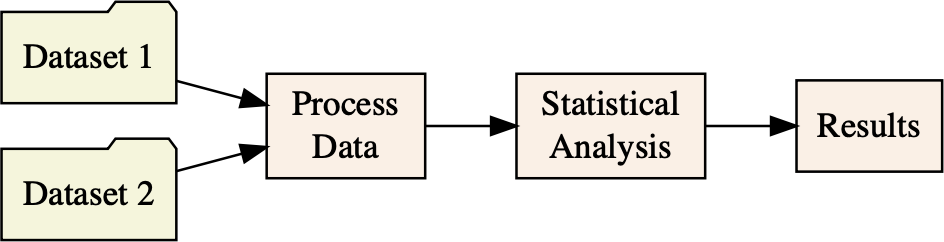
\includegraphics{bookdown_files/figure-latex/流程图-1.png}

\hypertarget{section-9}{%
\chapter{参数估计}\label{section-9}}

对于参数估计的模拟,主要分成三步:

\begin{enumerate}
\def\labelenumi{\arabic{enumi}.}
\tightlist
\item
  生成数据;
\item
  估计参数;
\item
  评价估计好坏.
\end{enumerate}

对于生成数据,在阅读文献时,文章中会明确给出如何产生.我们不必多费周折.在设计我们自己的模拟实验时,多借鉴其他文献中的例子.一方面方便和其他文献进行比较,另一方面,可以避免落入陷阱\footnote{程序在 \href{\%22code/Rcpp-demo.cpp\%22}{这里} 查看,其中最后被/***R */夹住的部分是R程序,每次加载后会自动执行,方便调试.}.

对于评价估计好坏,有限维离散参数一般采取\(\left\|\hat{\boldsymbol{\theta}}-\boldsymbol{\theta}_{0}\right\|,\)无穷维函数一般采取\(\int\left(\hat{m}(x)-m_{0}(x)\right)^{2} d x.\)

估计量通过解估计方程得到,根据方程的形式,分为M估计量和Z估计量,下面分别说明.

\hypertarget{m}{%
\section{M估计}\label{m}}

定义:极大化(或极小化)目标函数得到参数估计值.

\[
M_{n}(\theta)=\frac{1}{n} \sum_{i=1}^{n} m_{\theta}\left(X_{i}\right)
\]

\[
\hat{\theta}=\arg \max_{\theta \in \Theta} M_{n}(\theta)
\]

其中\(m_{\theta}\left(X_{i}\right)\)为已知函数.特别的,如果\(M_n(\theta)\)可导,M估计量和Z估计量有等价形式.

下面以线性模型为例:\(\boldsymbol{Y}=\boldsymbol{X}^{T}\boldsymbol{\theta}+\boldsymbol{\varepsilon}\)

考虑最小二乘估计,取\(m_{\theta}\left(\boldsymbol{X}_{i}\right)=-\left(Y_{i}-\boldsymbol{X}_{i}^{T} \boldsymbol{\theta}\right)^{2}\)\footnote{垃圾回收(英语:Garbage Collection,缩写为GC),在计算机科学中是一种自动的存储器管理机制。当一个计算机上的动态存储器不再需要时,就应该予以释放,以让出存储器,这种存储器资源管理,称为垃圾回收。},则

\[ 
\begin{aligned} 
M_{n}(\theta)&=-\frac{1}{n} \sum_{i=1}^{n}\left(Y_{i}-\boldsymbol{X}_{i}^{T} \boldsymbol{\theta}\right)^{2}\\
&=-\frac{1}{n}\left(\boldsymbol{Y}-\boldsymbol{X}^{T} \boldsymbol{\theta}\right)^{T}\left(\boldsymbol{Y}-\boldsymbol{X}^{T} \boldsymbol{\theta}\right)\\
&=-\frac{1}{n}\left(\boldsymbol{\theta}^{T} \boldsymbol{X} \boldsymbol{X}^{T} \boldsymbol{\theta}-2 \boldsymbol{Y}^{T} \boldsymbol{X}^{T} \boldsymbol{\theta}+\boldsymbol{Y}^{T} \boldsymbol{Y}\right)
\end{aligned} 
\]
其中最后一项是与\(\boldsymbol{\theta}\)无关的常数项,可以不考虑,进而可以整理成如下的二次规划问题:

利用quadprog包中的函数可以求解

\begin{Shaded}
\begin{Highlighting}[]
\KeywordTok{library}\NormalTok{(quadprog)}
\NormalTok{n=}\DecValTok{100}\NormalTok{;p=}\DecValTok{3}\NormalTok{;beta=}\KeywordTok{c}\NormalTok{(}\DecValTok{1}\NormalTok{,}\OperatorTok{-}\DecValTok{2}\NormalTok{,}\DecValTok{3}\NormalTok{);}
\NormalTok{X =}\StringTok{ }\KeywordTok{matrix}\NormalTok{(}\KeywordTok{rnorm}\NormalTok{(n}\OperatorTok{*}\NormalTok{p),n,p)}
\NormalTok{Y =}\StringTok{ }\NormalTok{X}\OperatorTok\NormalTok{beta }\OperatorTok{+}\StringTok{ }\KeywordTok{rnorm}\NormalTok{(n)}
\KeywordTok{lm}\NormalTok{(Y}\OperatorTok{~}\NormalTok{X}\OperatorTok{+}\DecValTok{0}\NormalTok{)}\OperatorTok{$}\NormalTok{coef }\OperatorTok{==}\StringTok{ }\KeywordTok{solve.QP}\NormalTok{(}\DataTypeTok{Dmat =} \KeywordTok{t}\NormalTok{(X)}\OperatorTok\NormalTok{X}\OperatorTok{/}\NormalTok{n, }\DataTypeTok{dvec =}\NormalTok{ (}\KeywordTok{t}\NormalTok{(Y)}\OperatorTok\NormalTok{X)}\OperatorTok{/}\NormalTok{n, }\DataTypeTok{Amat =} \KeywordTok{matrix}\NormalTok{(}\DecValTok{0}\NormalTok{,p,p))}\OperatorTok{$}\NormalTok{solution}
\end{Highlighting}
\end{Shaded}

\begin{verbatim}
##    X1    X2    X3 
## FALSE FALSE FALSE
\end{verbatim}

可以看到结果显示不相等,但是如果我们打印出来显示:

\begin{Shaded}
\begin{Highlighting}[]
\KeywordTok{lm}\NormalTok{(Y}\OperatorTok{~}\NormalTok{X}\OperatorTok{+}\DecValTok{0}\NormalTok{)}\OperatorTok{$}\NormalTok{coef}
\end{Highlighting}
\end{Shaded}

\begin{verbatim}
##      X1      X2      X3 
##  0.9307 -2.0048  2.8726
\end{verbatim}

\begin{Shaded}
\begin{Highlighting}[]
\KeywordTok{solve.QP}\NormalTok{(}\DataTypeTok{Dmat =} \KeywordTok{t}\NormalTok{(X)}\OperatorTok\NormalTok{X}\OperatorTok{/}\NormalTok{n, }\DataTypeTok{dvec =}\NormalTok{ (}\KeywordTok{t}\NormalTok{(Y)}\OperatorTok\NormalTok{X)}\OperatorTok{/}\NormalTok{n, }\DataTypeTok{Amat =} \KeywordTok{matrix}\NormalTok{(}\DecValTok{0}\NormalTok{,p,p))}\OperatorTok{$}\NormalTok{solution}
\end{Highlighting}
\end{Shaded}

\begin{verbatim}
## [1]  0.9307 -2.0048  2.8726
\end{verbatim}

可以看到结果是一致的.这是由于计算机存储数字精度引起的.比如我们查看

\begin{Shaded}
\begin{Highlighting}[]
\KeywordTok{sum}\NormalTok{(}\KeywordTok{abs}\NormalTok{(}\KeywordTok{lm}\NormalTok{(Y}\OperatorTok{~}\NormalTok{X}\OperatorTok{+}\DecValTok{0}\NormalTok{)}\OperatorTok{$}\NormalTok{coef }\OperatorTok{-}
\KeywordTok{solve.QP}\NormalTok{(}\DataTypeTok{Dmat =} \KeywordTok{t}\NormalTok{(X)}\OperatorTok\NormalTok{X}\OperatorTok{/}\NormalTok{n, }\DataTypeTok{dvec =}\NormalTok{ (}\KeywordTok{t}\NormalTok{(Y)}\OperatorTok\NormalTok{X)}\OperatorTok{/}\NormalTok{n, }\DataTypeTok{Amat =} \KeywordTok{matrix}\NormalTok{(}\DecValTok{0}\NormalTok{,p,p))}\OperatorTok{$}\NormalTok{solution))}
\end{Highlighting}
\end{Shaded}

\begin{verbatim}
## [1] 4.552e-15
\end{verbatim}

另外,我们可以用all.equal这个函数设置容忍的误差值,判断近似相等:

\begin{Shaded}
\begin{Highlighting}[]
\KeywordTok{all.equal}\NormalTok{(}\KeywordTok{unname}\NormalTok{(}\KeywordTok{lm}\NormalTok{(Y}\OperatorTok{~}\NormalTok{X}\OperatorTok{+}\DecValTok{0}\NormalTok{)}\OperatorTok{$}\NormalTok{coef),}
\KeywordTok{solve.QP}\NormalTok{(}\DataTypeTok{Dmat =} \KeywordTok{t}\NormalTok{(X)}\OperatorTok\NormalTok{X}\OperatorTok{/}\NormalTok{n, }\DataTypeTok{dvec =}\NormalTok{ (}\KeywordTok{t}\NormalTok{(Y)}\OperatorTok\NormalTok{X)}\OperatorTok{/}\NormalTok{n, }\DataTypeTok{Amat =} \KeywordTok{matrix}\NormalTok{(}\DecValTok{0}\NormalTok{,p,p))}\OperatorTok{$}\NormalTok{solution}
\NormalTok{,}\DataTypeTok{tolerance=}\FloatTok{1e-10}\NormalTok{)}
\end{Highlighting}
\end{Shaded}

\begin{verbatim}
## [1] TRUE
\end{verbatim}

\begin{Shaded}
\begin{Highlighting}[]
\KeywordTok{all.equal}\NormalTok{(}\KeywordTok{unname}\NormalTok{(}\KeywordTok{lm}\NormalTok{(Y}\OperatorTok{~}\NormalTok{X}\OperatorTok{+}\DecValTok{0}\NormalTok{)}\OperatorTok{$}\NormalTok{coef),}
\KeywordTok{solve.QP}\NormalTok{(}\DataTypeTok{Dmat =} \KeywordTok{t}\NormalTok{(X)}\OperatorTok\NormalTok{X}\OperatorTok{/}\NormalTok{n, }\DataTypeTok{dvec =}\NormalTok{ (}\KeywordTok{t}\NormalTok{(Y)}\OperatorTok\NormalTok{X)}\OperatorTok{/}\NormalTok{n, }\DataTypeTok{Amat =} \KeywordTok{matrix}\NormalTok{(}\DecValTok{0}\NormalTok{,p,p))}\OperatorTok{$}\NormalTok{solution}
\NormalTok{,}\DataTypeTok{tolerance=}\FloatTok{1e-20}\NormalTok{)}
\end{Highlighting}
\end{Shaded}

\begin{verbatim}
## [1] "Mean relative difference: 7.837e-16"
\end{verbatim}

下面考虑稍复杂的情况,取
\(m_{\theta}\left(\boldsymbol{X}_{i}\right)=\rho_{\tau}\left(y_{i}-\boldsymbol{X}_{i}^{T} \boldsymbol{\theta}\right)\),其中
\(\rho_{\tau}(t)=t\left(\tau-I_{\{t<0\}}\right)\).
这称为分位数回归,详细的推导过程可以在\href{https://github.com/dujiangbjut/dujiangbjut.github.io/tree/master/讨论班/分位数回归}{分位数回归总结}查看\footnote{后续重新整理成Rmd格式.}.

\textbf{这里缺少一个M估计迭代求解的例子}

\hypertarget{z}{%
\section{Z估计}\label{z}}

定义:解一个等于0的方程得到参数估计.

\[
\Psi_{n}(\theta)=\frac{1}{n} \sum_{i=1}^{n} \psi_{\theta}\left(X_{i}\right)=0,
\]
其中\(\psi_{\theta}\left(X_{i}\right)\)为已知函数.

\(\hat{\theta}\)为
\(\Psi_{n}(\theta)=0\)的解.

回到线性模型最小二乘的例子,由于目标函数存在导数,可以转化成一个Z估计量.取
\(\psi_{\theta}\left(X_{i}\right)=m_{\theta}'\left(X_{i}\right)=2\boldsymbol{X}_{i}^{T} \left(Y_{i}-\boldsymbol{X}_{i}^{T} \boldsymbol{\theta}\right)\)

则\footnote{省略了常数系数.}
\[
\Psi_{n}(\theta)=\frac{1}{n} \sum_{i=1}^{n}\boldsymbol{X}_{i}^{T}  \left(Y_{i}-\boldsymbol{X}_{i}^{T} \boldsymbol{\theta}\right) =\boldsymbol{X} \boldsymbol{X}^{T} \boldsymbol{\theta}-\boldsymbol{X} \boldsymbol{Y}=0,
\]

进而得到参数估计值为:\(\hat{\boldsymbol{\theta}}=\left(\boldsymbol{X} \boldsymbol{X}^{T}\right)^{-1} \boldsymbol{X} \boldsymbol{Y}.\)

通过下面的程序验证:

\begin{Shaded}
\begin{Highlighting}[]
\KeywordTok{library}\NormalTok{(quadprog)}
\KeywordTok{all.equal}\NormalTok{(}\KeywordTok{solve.QP}\NormalTok{(}\DataTypeTok{Dmat =} \KeywordTok{t}\NormalTok{(X)}\OperatorTok\NormalTok{X}\OperatorTok{/}\NormalTok{n, }\DataTypeTok{dvec =}\NormalTok{ (}\KeywordTok{t}\NormalTok{(Y)}\OperatorTok\NormalTok{X)}\OperatorTok{/}\NormalTok{n, }\DataTypeTok{Amat =} \KeywordTok{matrix}\NormalTok{(}\DecValTok{0}\NormalTok{,p,p))}\OperatorTok{$}\NormalTok{solution, }\KeywordTok{as.numeric}\NormalTok{(}\KeywordTok{solve}\NormalTok{(}\KeywordTok{t}\NormalTok{(X)}\OperatorTok\NormalTok{X)}\OperatorTok\KeywordTok{t}\NormalTok{(X)}\OperatorTok\NormalTok{Y))}
\end{Highlighting}
\end{Shaded}

\begin{verbatim}
## [1] TRUE
\end{verbatim}

下面是一个迭代求解Z估计量的例子\footnote{目前只有单次二项分布的程序正确.完整的程序可以从\href{code/glm.R}{这里}下载.}.

\textbf{补充哪一篇参考文献}

\begin{Shaded}
\begin{Highlighting}[]
\KeywordTok{source}\NormalTok{(}\StringTok{"code/glm.R"}\NormalTok{)}
\NormalTok{n=}\DecValTok{500}
\NormalTok{m1=}\DecValTok{2}
\NormalTok{m2=}\DecValTok{2}
\NormalTok{m3=}\DecValTok{2}
\NormalTok{m=m1}\OperatorTok{+}\NormalTok{m2}\OperatorTok{+}\NormalTok{m3}
\NormalTok{beta=}\KeywordTok{c}\NormalTok{(}\KeywordTok{rep}\NormalTok{(}\OperatorTok{-}\DecValTok{1}\NormalTok{,m1),}\KeywordTok{rep}\NormalTok{(}\DecValTok{0}\NormalTok{,m2),}\KeywordTok{rep}\NormalTok{(}\DecValTok{1}\NormalTok{,m3))}
\NormalTok{X=}\KeywordTok{runif}\NormalTok{(n}\OperatorTok{*}\NormalTok{m,}\OperatorTok{-}\DecValTok{1}\NormalTok{,}\DecValTok{1}\NormalTok{)}
\NormalTok{X=}\KeywordTok{matrix}\NormalTok{(X,n,m)}
\NormalTok{eta=X}\OperatorTok\NormalTok{beta}
\NormalTok{mu=}\DecValTok{1}\OperatorTok{/}\NormalTok{(}\DecValTok{1}\OperatorTok{+}\KeywordTok{exp}\NormalTok{(}\OperatorTok{-}\NormalTok{eta))}

\CommentTok{# Y~B(1,p)}
\NormalTok{Y=}\KeywordTok{runif}\NormalTok{(n)}
\NormalTok{Y[Y}\OperatorTok{>=}\NormalTok{mu]=}\DecValTok{0}
\NormalTok{Y[Y}\OperatorTok{>}\DecValTok{0}\NormalTok{]=}\DecValTok{1}
\KeywordTok{glm}\NormalTok{(Y}\OperatorTok{~}\NormalTok{X}\OperatorTok{+}\DecValTok{0}\NormalTok{,}\DataTypeTok{family=}\KeywordTok{binomial}\NormalTok{(}\DataTypeTok{link=}\StringTok{"logit"}\NormalTok{))}
\end{Highlighting}
\end{Shaded}

\begin{verbatim}
## 
## Call:  glm(formula = Y ~ X + 0, family = binomial(link = "logit"))
## 
## Coefficients:
##      X1       X2       X3       X4       X5       X6  
## -0.9136  -1.0812   0.1308   0.0902   0.8542   0.5147  
## 
## Degrees of Freedom: 500 Total (i.e. Null);  494 Residual
## Null Deviance:       693 
## Residual Deviance: 593   AIC: 605
\end{verbatim}

\begin{Shaded}
\begin{Highlighting}[]
\KeywordTok{myglm}\NormalTok{(Y,X,}\DataTypeTok{distribution  =} \StringTok{"binom"}\NormalTok{)}
\end{Highlighting}
\end{Shaded}

\begin{verbatim}
## $theta
##          [,1]
## [1,] -0.93491
## [2,] -1.11849
## [3,]  0.11274
## [4,]  0.09284
## [5,]  0.87808
## [6,]  0.52674
## 
## $steps
## [1] 5
\end{verbatim}

可以看到和真值相差不大,但是很快收敛.

\hypertarget{section-10}{%
\chapter{假设检验}\label{section-10}}

假设检验部分模拟相对简单,只需要在估计出参数值后,按照检验统计量的形式正确计算即可.主要难点在于构造检验统计量以及给出检验统计量的渐近分布.

常用的办法是通过自助法(bootstrap)估计分布.

我们以最简单的二项分布为例,说明一些假设检验中的概念.

\begin{tabular}{r|r|r|r|r|r}
\hline
X & p=0.5 & p=0.6 & p=0.7 & p=0.8 & p=0.9\\
\hline
0 & 0.0010 & 0.0001 & 0.0000 & 0.0000 & 0.0000\\
\hline
1 & 0.0098 & 0.0016 & 0.0001 & 0.0000 & 0.0000\\
\hline
2 & 0.0439 & 0.0106 & 0.0014 & 0.0001 & 0.0000\\
\hline
3 & 0.1172 & 0.0425 & 0.0090 & 0.0008 & 0.0000\\
\hline
4 & 0.2051 & 0.1115 & 0.0368 & 0.0055 & 0.0001\\
\hline
5 & 0.2461 & 0.2007 & 0.1029 & 0.0264 & 0.0015\\
\hline
6 & 0.2051 & 0.2508 & 0.2001 & 0.0881 & 0.0112\\
\hline
7 & 0.1172 & 0.2150 & 0.2668 & 0.2013 & 0.0574\\
\hline
8 & 0.0439 & 0.1209 & 0.2335 & 0.3020 & 0.1937\\
\hline
9 & 0.0098 & 0.0403 & 0.1211 & 0.2684 & 0.3874\\
\hline
10 & 0.0010 & 0.0060 & 0.0282 & 0.1074 & 0.3487\\
\hline
\end{tabular}

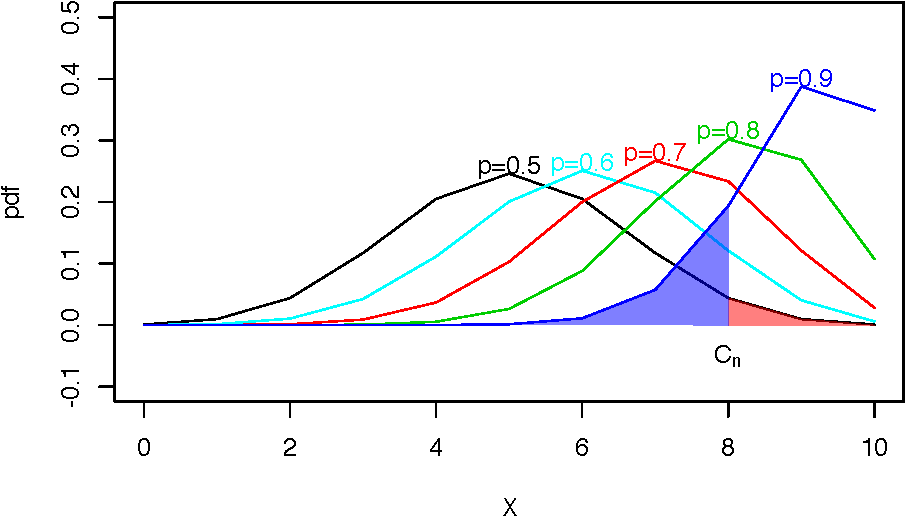
\includegraphics{bookdown_files/figure-latex/unnamed-chunk-25-1.pdf}

显著水平=第一类错误=\(\alpha\):为图中红色区域的面积

第二类错误=\(\beta\):为图中蓝色区域的面积

功效=势=power=\(1- \beta\):为图中蓝色曲线下空白面积

检验的相合性:

\begin{enumerate}
\def\labelenumi{\arabic{enumi}.}
\tightlist
\item
  在\(H_0\)下, 拒绝概率(size)收敛到\(\alpha.\)
\item
  在\(H_1\)下, 拒绝概率(power)收敛到\(1.\)
\end{enumerate}

\hypertarget{section-11}{%
\chapter{进阶技巧}\label{section-11}}

程序的可读性和执行效率是两个很重要的要求.这一章主要介绍如何提高这两点.

\hypertarget{apply}{%
\section{apply函数族}\label{apply}}

\textbf{apply并不能提高执行效率,只能使代码简洁易读.}

详细的介绍可以在\href{http://blog.fens.me/r-apply/}{apply函数族介绍}查看,其中给了一些简单的例子.下面演示一下稍微复杂的用法.

对矩阵按列进行操作,每列的奇数项求和,偶数项求和:

\begin{Shaded}
\begin{Highlighting}[]
\NormalTok{m <-}\StringTok{ }\KeywordTok{matrix}\NormalTok{(}\DecValTok{1}\OperatorTok{:}\DecValTok{12}\NormalTok{,}\DecValTok{4}\NormalTok{,}\DecValTok{3}\NormalTok{)}
\NormalTok{m}
\end{Highlighting}
\end{Shaded}

\begin{verbatim}
##      [,1] [,2] [,3]
## [1,]    1    5    9
## [2,]    2    6   10
## [3,]    3    7   11
## [4,]    4    8   12
\end{verbatim}

\begin{Shaded}
\begin{Highlighting}[]
\KeywordTok{apply}\NormalTok{(m, }\DecValTok{2}\NormalTok{, tapply,}\KeywordTok{rep}\NormalTok{(}\DecValTok{1}\OperatorTok{:}\DecValTok{2}\NormalTok{,}\DecValTok{2}\NormalTok{), sum)}
\end{Highlighting}
\end{Shaded}

\begin{verbatim}
##   [,1] [,2] [,3]
## 1    4   12   20
## 2    6   14   22
\end{verbatim}

对矩阵按列进行操作,每列前两项求和,后两项求和:

\begin{Shaded}
\begin{Highlighting}[]
\KeywordTok{apply}\NormalTok{(m, }\DecValTok{2}\NormalTok{, tapply,}\KeywordTok{rep}\NormalTok{(}\DecValTok{1}\OperatorTok{:}\DecValTok{2}\NormalTok{,}\DataTypeTok{each=}\DecValTok{2}\NormalTok{), sum)}
\end{Highlighting}
\end{Shaded}

\begin{verbatim}
##   [,1] [,2] [,3]
## 1    3   11   19
## 2    7   15   23
\end{verbatim}

下面看一个3维情况的例子.

\begin{Shaded}
\begin{Highlighting}[]
\NormalTok{a <-}\StringTok{ }\KeywordTok{array}\NormalTok{(}\DecValTok{1}\OperatorTok{:}\DecValTok{24}\NormalTok{,}\DataTypeTok{dim =} \KeywordTok{c}\NormalTok{(}\DecValTok{2}\NormalTok{,}\DecValTok{3}\NormalTok{,}\DecValTok{4}\NormalTok{))}
\NormalTok{a}
\end{Highlighting}
\end{Shaded}

\begin{verbatim}
## , , 1
## 
##      [,1] [,2] [,3]
## [1,]    1    3    5
## [2,]    2    4    6
## 
## , , 2
## 
##      [,1] [,2] [,3]
## [1,]    7    9   11
## [2,]    8   10   12
## 
## , , 3
## 
##      [,1] [,2] [,3]
## [1,]   13   15   17
## [2,]   14   16   18
## 
## , , 4
## 
##      [,1] [,2] [,3]
## [1,]   19   21   23
## [2,]   20   22   24
\end{verbatim}

固定1个维度,对另外2个维度求和:

\begin{Shaded}
\begin{Highlighting}[]
\KeywordTok{apply}\NormalTok{(a,}\DecValTok{1}\NormalTok{,sum)}
\end{Highlighting}
\end{Shaded}

\begin{verbatim}
## [1] 144 156
\end{verbatim}

这样看起来不太直观,我们利用aperm函数调整数组的维度顺序:

\begin{Shaded}
\begin{Highlighting}[]
\KeywordTok{aperm}\NormalTok{(a,}\KeywordTok{c}\NormalTok{(}\DecValTok{2}\NormalTok{,}\DecValTok{3}\NormalTok{,}\DecValTok{1}\NormalTok{))}
\end{Highlighting}
\end{Shaded}

\begin{verbatim}
## , , 1
## 
##      [,1] [,2] [,3] [,4]
## [1,]    1    7   13   19
## [2,]    3    9   15   21
## [3,]    5   11   17   23
## 
## , , 2
## 
##      [,1] [,2] [,3] [,4]
## [1,]    2    8   14   20
## [2,]    4   10   16   22
## [3,]    6   12   18   24
\end{verbatim}

固定2个维度,对1个维度求和:

\begin{Shaded}
\begin{Highlighting}[]
\KeywordTok{apply}\NormalTok{(a,}\KeywordTok{c}\NormalTok{(}\DecValTok{2}\NormalTok{,}\DecValTok{3}\NormalTok{),sum)}
\end{Highlighting}
\end{Shaded}

\begin{verbatim}
##      [,1] [,2] [,3] [,4]
## [1,]    3   15   27   39
## [2,]    7   19   31   43
## [3,]   11   23   35   47
\end{verbatim}

固定2个维度,对1个维度分组求和:

\begin{Shaded}
\begin{Highlighting}[]
\KeywordTok{apply}\NormalTok{(a,}\KeywordTok{c}\NormalTok{(}\DecValTok{1}\NormalTok{,}\DecValTok{2}\NormalTok{),tapply,}\KeywordTok{rep}\NormalTok{(}\KeywordTok{c}\NormalTok{(}\OperatorTok{-}\DecValTok{1}\NormalTok{,}\OperatorTok{-}\DecValTok{2}\NormalTok{),}\DecValTok{2}\NormalTok{), sum)}
\end{Highlighting}
\end{Shaded}

\begin{verbatim}
## , , 1
## 
##    [,1] [,2]
## -2   26   28
## -1   14   16
## 
## , , 2
## 
##    [,1] [,2]
## -2   30   32
## -1   18   20
## 
## , , 3
## 
##    [,1] [,2]
## -2   34   36
## -1   22   24
\end{verbatim}

对第三个维度奇数项、偶数项分别求和(奇数项是-1组,偶数项是-2组).

\hypertarget{section-12}{%
\section{并行}\label{section-12}}

\textbf{单次模拟时间越长,重复次数越多,并行得到的提升越明显.}

R中有很多并行包,可以在
\href{https://yulongniu.bionutshell.org/blog/2014/06/25/parallel-package/}{不同并行包比较}查看对比.

这里介绍的foreach是比较友好的一个包.

下面以线性模型估计系数为例,给出示例代码.

sim\_single可以在
\href{\%22code/parallel-demo.R\%22}{单次估计程序}
查看.其中SLP参数用于增加单次模拟的计算量(运行时间).

\hypertarget{section-13}{%
\subsection{低重复次数,低计算量}\label{section-13}}

\begin{Shaded}
\begin{Highlighting}[]
\KeywordTok{source}\NormalTok{(}\StringTok{"code/parallel-demo.R"}\NormalTok{)}
\KeywordTok{library}\NormalTok{(}\StringTok{"foreach"}\NormalTok{)}
\KeywordTok{library}\NormalTok{(}\StringTok{"doParallel"}\NormalTok{)}
\NormalTok{beta0 =}\StringTok{ }\KeywordTok{c}\NormalTok{(}\DecValTok{1}\NormalTok{,}\OperatorTok{-}\DecValTok{2}\NormalTok{,}\DecValTok{3}\NormalTok{)}
\NormalTok{N =}\StringTok{ }\KeywordTok{c}\NormalTok{(}\DecValTok{50}\NormalTok{,}\DecValTok{100}\NormalTok{,}\DecValTok{200}\NormalTok{)}
\NormalTok{distribution=}\StringTok{ }\KeywordTok{c}\NormalTok{(rnorm,rcauchy)}
\NormalTok{SIM =}\StringTok{ }\DecValTok{500}
\NormalTok{tstart=}\KeywordTok{Sys.time}\NormalTok{()}
\NormalTok{cl <-}\StringTok{ }\KeywordTok{makeCluster}\NormalTok{(}\KeywordTok{detectCores}\NormalTok{())}
\KeywordTok{registerDoParallel}\NormalTok{(cl)}
\NormalTok{result <-}\StringTok{ }\KeywordTok{foreach}\NormalTok{(}\DataTypeTok{n=}\NormalTok{N,}\DataTypeTok{.combine =}\NormalTok{ rbind) }\OperatorTok
\StringTok{  }\KeywordTok{foreach}\NormalTok{(}\DataTypeTok{dst=}\NormalTok{distribution,}\DataTypeTok{.combine =}\NormalTok{ c) }\OperatorTok
\StringTok{  }\KeywordTok{foreach}\NormalTok{(}\DataTypeTok{i=}\DecValTok{1}\OperatorTok{:}\NormalTok{SIM,}\DataTypeTok{.combine =} \StringTok{'+'}\NormalTok{,}
          \DataTypeTok{.packages =} \KeywordTok{c}\NormalTok{(}\StringTok{"MASS"}\NormalTok{) )}\OperatorTok\NormalTok{\{}
            \KeywordTok{sim_single}\NormalTok{(n,beta0,}\DataTypeTok{SLP=}\OtherTok{FALSE}\NormalTok{,}\DataTypeTok{mydist =}\NormalTok{ dst)}
\NormalTok{          \}}
\KeywordTok{stopImplicitCluster}\NormalTok{()}
\NormalTok{t.end=}\KeywordTok{Sys.time}\NormalTok{()}
\NormalTok{t.end}\OperatorTok{-}\NormalTok{tstart}
\end{Highlighting}
\end{Shaded}

\begin{verbatim}
## Time difference of 2.154 secs
\end{verbatim}

\begin{Shaded}
\begin{Highlighting}[]
\NormalTok{result}\OperatorTok{/}\NormalTok{SIM}
\end{Highlighting}
\end{Shaded}

\begin{verbatim}
##           [,1]   [,2]  [,3]    [,4]   [,5]   [,6]
## result.1 1.003 -2.001 3.005 -1.1727 -2.584 -2.439
## result.2 1.004 -2.001 3.001  1.2478 -1.499  1.550
## result.3 1.002 -2.003 3.001  0.8456 -2.193  2.800
\end{verbatim}

把申请cluster的命令去掉,\%dopar\%换成\%do\%程序就会按串行执行

\begin{Shaded}
\begin{Highlighting}[]
\KeywordTok{source}\NormalTok{(}\StringTok{"code/parallel-demo.R"}\NormalTok{)}
\KeywordTok{library}\NormalTok{(}\StringTok{"foreach"}\NormalTok{)}
\KeywordTok{library}\NormalTok{(}\StringTok{"doParallel"}\NormalTok{)}
\NormalTok{beta0 =}\StringTok{  }\KeywordTok{c}\NormalTok{(}\DecValTok{1}\NormalTok{,}\OperatorTok{-}\DecValTok{2}\NormalTok{,}\DecValTok{3}\NormalTok{)}
\NormalTok{N =}\StringTok{ }\KeywordTok{c}\NormalTok{(}\DecValTok{50}\NormalTok{,}\DecValTok{100}\NormalTok{,}\DecValTok{200}\NormalTok{)}
\NormalTok{distribution=}\StringTok{ }\KeywordTok{c}\NormalTok{(rnorm,rcauchy)}
\NormalTok{SIM =}\StringTok{ }\DecValTok{500}
\NormalTok{tstart=}\KeywordTok{Sys.time}\NormalTok{()}
\CommentTok{#cl <- makeCluster(detectCores())}
\CommentTok{#registerDoParallel(cl)}
\NormalTok{result <-}\StringTok{ }\KeywordTok{foreach}\NormalTok{(}\DataTypeTok{n=}\NormalTok{N,}\DataTypeTok{.combine =}\NormalTok{ rbind) }\OperatorTok
\StringTok{  }\KeywordTok{foreach}\NormalTok{(}\DataTypeTok{dst=}\NormalTok{distribution,}\DataTypeTok{.combine =}\NormalTok{ c) }\OperatorTok
\StringTok{  }\KeywordTok{foreach}\NormalTok{(}\DataTypeTok{i=}\DecValTok{1}\OperatorTok{:}\NormalTok{SIM,}\DataTypeTok{.combine =} \StringTok{'+'}\NormalTok{,}
          \DataTypeTok{.packages =} \KeywordTok{c}\NormalTok{(}\StringTok{"MASS"}\NormalTok{) )}\OperatorTok\NormalTok{\{}
            \KeywordTok{sim_single}\NormalTok{(n,beta0,}\DataTypeTok{SLP=}\OtherTok{FALSE}\NormalTok{,}\DataTypeTok{mydist =}\NormalTok{ dst)}
\NormalTok{          \}}
\CommentTok{#stopImplicitCluster()}
\NormalTok{t.end=}\KeywordTok{Sys.time}\NormalTok{()}
\NormalTok{t.end}\OperatorTok{-}\NormalTok{tstart}
\end{Highlighting}
\end{Shaded}

\begin{verbatim}
## Time difference of 2.286 secs
\end{verbatim}

\begin{Shaded}
\begin{Highlighting}[]
\NormalTok{result}\OperatorTok{/}\NormalTok{SIM}
\end{Highlighting}
\end{Shaded}

\begin{verbatim}
##            [,1]   [,2]  [,3]   [,4]   [,5]   [,6]
## result.1 1.0122 -2.005 3.004 -1.917 -2.588 -3.872
## result.2 0.9973 -2.003 2.994 -2.835 -6.775 -2.712
## result.3 1.0041 -2.005 2.995  1.019 -2.212  2.953
\end{verbatim}

\hypertarget{section-14}{%
\subsection{高重复次数,低计算量}\label{section-14}}

增加到1000次.

并行:

\begin{Shaded}
\begin{Highlighting}[]
\KeywordTok{source}\NormalTok{(}\StringTok{"/Users/wang/Documents/GitHub/Simulation-in-R/code/parallel-demo.R"}\NormalTok{)}
\KeywordTok{library}\NormalTok{(}\StringTok{"foreach"}\NormalTok{)}
\KeywordTok{library}\NormalTok{(}\StringTok{"doParallel"}\NormalTok{)}
\NormalTok{beta0 =}\StringTok{ }\KeywordTok{c}\NormalTok{(}\DecValTok{1}\NormalTok{,}\OperatorTok{-}\DecValTok{2}\NormalTok{,}\DecValTok{3}\NormalTok{)}
\NormalTok{N =}\StringTok{ }\KeywordTok{c}\NormalTok{(}\DecValTok{50}\NormalTok{,}\DecValTok{100}\NormalTok{,}\DecValTok{200}\NormalTok{)}
\NormalTok{distribution=}\StringTok{ }\KeywordTok{c}\NormalTok{(rnorm,rcauchy)}
\NormalTok{SIM =}\StringTok{ }\DecValTok{1000}
\NormalTok{tstart=}\KeywordTok{Sys.time}\NormalTok{()}
\NormalTok{cl <-}\StringTok{ }\KeywordTok{makeCluster}\NormalTok{(}\KeywordTok{detectCores}\NormalTok{())}
\KeywordTok{registerDoParallel}\NormalTok{(cl)}
\NormalTok{result <-}\StringTok{ }\KeywordTok{foreach}\NormalTok{(}\DataTypeTok{n=}\NormalTok{N,}\DataTypeTok{.combine =}\NormalTok{ rbind) }\OperatorTok
\StringTok{  }\KeywordTok{foreach}\NormalTok{(}\DataTypeTok{dst=}\NormalTok{distribution,}\DataTypeTok{.combine =}\NormalTok{ c) }\OperatorTok
\StringTok{  }\KeywordTok{foreach}\NormalTok{(}\DataTypeTok{i=}\DecValTok{1}\OperatorTok{:}\NormalTok{SIM,}\DataTypeTok{.combine =} \StringTok{'+'}\NormalTok{,}
          \DataTypeTok{.packages =} \KeywordTok{c}\NormalTok{(}\StringTok{"MASS"}\NormalTok{) )}\OperatorTok\NormalTok{\{}
            \KeywordTok{sim_single}\NormalTok{(n,beta0,}\DataTypeTok{SLP=}\OtherTok{FALSE}\NormalTok{,}\DataTypeTok{mydist =}\NormalTok{ dst)}
\NormalTok{          \}}
\KeywordTok{stopImplicitCluster}\NormalTok{()}
\NormalTok{t.end=}\KeywordTok{Sys.time}\NormalTok{()}
\NormalTok{t.end}\OperatorTok{-}\NormalTok{tstart}
\end{Highlighting}
\end{Shaded}

\begin{verbatim}
## Time difference of 3.242 secs
\end{verbatim}

\begin{Shaded}
\begin{Highlighting}[]
\NormalTok{result}\OperatorTok{/}\NormalTok{SIM}
\end{Highlighting}
\end{Shaded}

\begin{verbatim}
##            [,1]   [,2]  [,3]   [,4]   [,5]  [,6]
## result.1 1.0002 -2.002 3.007 2.1339 -1.191 4.508
## result.2 0.9987 -2.005 2.999 1.6117 -1.703 3.207
## result.3 1.0015 -2.001 2.999 0.9367 -1.038 2.027
\end{verbatim}

串行:

\begin{Shaded}
\begin{Highlighting}[]
\KeywordTok{source}\NormalTok{(}\StringTok{"code/parallel-demo.R"}\NormalTok{)}
\KeywordTok{library}\NormalTok{(}\StringTok{"foreach"}\NormalTok{)}
\KeywordTok{library}\NormalTok{(}\StringTok{"doParallel"}\NormalTok{)}
\NormalTok{beta0 =}\StringTok{  }\KeywordTok{c}\NormalTok{(}\DecValTok{1}\NormalTok{,}\OperatorTok{-}\DecValTok{2}\NormalTok{,}\DecValTok{3}\NormalTok{)}
\NormalTok{N =}\StringTok{ }\KeywordTok{c}\NormalTok{(}\DecValTok{50}\NormalTok{,}\DecValTok{100}\NormalTok{,}\DecValTok{200}\NormalTok{)}
\NormalTok{distribution=}\StringTok{ }\KeywordTok{c}\NormalTok{(rnorm,rcauchy)}
\NormalTok{SIM =}\StringTok{ }\DecValTok{1000}
\NormalTok{tstart=}\KeywordTok{Sys.time}\NormalTok{()}
\CommentTok{#cl <- makeCluster(detectCores())}
\CommentTok{#registerDoParallel(cl)}
\NormalTok{result <-}\StringTok{ }\KeywordTok{foreach}\NormalTok{(}\DataTypeTok{n=}\NormalTok{N,}\DataTypeTok{.combine =}\NormalTok{ rbind) }\OperatorTok
\StringTok{  }\KeywordTok{foreach}\NormalTok{(}\DataTypeTok{dst=}\NormalTok{distribution,}\DataTypeTok{.combine =}\NormalTok{ c) }\OperatorTok
\StringTok{  }\KeywordTok{foreach}\NormalTok{(}\DataTypeTok{i=}\DecValTok{1}\OperatorTok{:}\NormalTok{SIM,}\DataTypeTok{.combine =} \StringTok{'+'}\NormalTok{,}
          \DataTypeTok{.packages =} \KeywordTok{c}\NormalTok{(}\StringTok{"MASS"}\NormalTok{) )}\OperatorTok\NormalTok{\{}
            \KeywordTok{sim_single}\NormalTok{(n,beta0,}\DataTypeTok{SLP=}\OtherTok{FALSE}\NormalTok{,}\DataTypeTok{mydist =}\NormalTok{ dst)}
\NormalTok{          \}}
\CommentTok{#stopImplicitCluster()}
\NormalTok{t.end=}\KeywordTok{Sys.time}\NormalTok{()}
\NormalTok{t.end}\OperatorTok{-}\NormalTok{tstart}
\end{Highlighting}
\end{Shaded}

\begin{verbatim}
## Time difference of 4.531 secs
\end{verbatim}

\begin{Shaded}
\begin{Highlighting}[]
\NormalTok{result}\OperatorTok{/}\NormalTok{SIM}
\end{Highlighting}
\end{Shaded}

\begin{verbatim}
##            [,1]   [,2]  [,3]   [,4]   [,5]  [,6]
## result.1 0.9935 -2.006 3.001 0.8280 -1.304 2.702
## result.2 1.0012 -2.008 2.997 0.6967 -3.121 3.216
## result.3 0.9970 -2.002 2.999 0.7598 -2.071 2.580
\end{verbatim}

\hypertarget{section-15}{%
\subsection{低重复次数,高计算量}\label{section-15}}

增加每次模拟的计算量,延长单次模拟的时间.

并行:

\begin{Shaded}
\begin{Highlighting}[]
\KeywordTok{source}\NormalTok{(}\StringTok{"/Users/wang/Documents/GitHub/Simulation-in-R/code/parallel-demo.R"}\NormalTok{)}
\KeywordTok{library}\NormalTok{(}\StringTok{"foreach"}\NormalTok{)}
\KeywordTok{library}\NormalTok{(}\StringTok{"doParallel"}\NormalTok{)}
\NormalTok{beta0 =}\StringTok{ }\KeywordTok{c}\NormalTok{(}\DecValTok{1}\NormalTok{,}\OperatorTok{-}\DecValTok{2}\NormalTok{,}\DecValTok{3}\NormalTok{)}
\NormalTok{N =}\StringTok{ }\KeywordTok{c}\NormalTok{(}\DecValTok{50}\NormalTok{,}\DecValTok{100}\NormalTok{,}\DecValTok{200}\NormalTok{)}
\NormalTok{distribution=}\StringTok{ }\KeywordTok{c}\NormalTok{(rnorm,rcauchy)}
\NormalTok{SIM =}\StringTok{ }\DecValTok{500}
\NormalTok{tstart=}\KeywordTok{Sys.time}\NormalTok{()}
\NormalTok{cl <-}\StringTok{ }\KeywordTok{makeCluster}\NormalTok{(}\KeywordTok{detectCores}\NormalTok{())}
\KeywordTok{registerDoParallel}\NormalTok{(cl)}
\NormalTok{result <-}\StringTok{ }\KeywordTok{foreach}\NormalTok{(}\DataTypeTok{n=}\NormalTok{N,}\DataTypeTok{.combine =}\NormalTok{ rbind) }\OperatorTok
\StringTok{  }\KeywordTok{foreach}\NormalTok{(}\DataTypeTok{dst=}\NormalTok{distribution,}\DataTypeTok{.combine =}\NormalTok{ c) }\OperatorTok
\StringTok{  }\KeywordTok{foreach}\NormalTok{(}\DataTypeTok{i=}\DecValTok{1}\OperatorTok{:}\NormalTok{SIM,}\DataTypeTok{.combine =} \StringTok{'+'}\NormalTok{,}
          \DataTypeTok{.packages =} \KeywordTok{c}\NormalTok{(}\StringTok{"MASS"}\NormalTok{) )}\OperatorTok\NormalTok{\{}
            \KeywordTok{sim_single}\NormalTok{(n,beta0,}\DataTypeTok{SLP=}\OtherTok{TRUE}\NormalTok{,}\DataTypeTok{mydist =}\NormalTok{ dst)}
\NormalTok{          \}}
\KeywordTok{stopImplicitCluster}\NormalTok{()}
\NormalTok{t.end=}\KeywordTok{Sys.time}\NormalTok{()}
\NormalTok{t.end}\OperatorTok{-}\NormalTok{tstart}
\end{Highlighting}
\end{Shaded}

\begin{verbatim}
## Time difference of 8.959 secs
\end{verbatim}

\begin{Shaded}
\begin{Highlighting}[]
\NormalTok{result}\OperatorTok{/}\NormalTok{SIM}
\end{Highlighting}
\end{Shaded}

\begin{verbatim}
##            [,1]   [,2]  [,3]   [,4]   [,5]  [,6]
## result.1 1.0022 -2.002 2.994 0.8619 -1.743 2.295
## result.2 1.0016 -2.011 3.003 1.5220 -3.314 2.860
## result.3 0.9994 -2.004 3.002 0.9241 -2.217 3.344
\end{verbatim}

串行:

\begin{Shaded}
\begin{Highlighting}[]
\KeywordTok{source}\NormalTok{(}\StringTok{"code/parallel-demo.R"}\NormalTok{)}
\KeywordTok{library}\NormalTok{(}\StringTok{"foreach"}\NormalTok{)}
\KeywordTok{library}\NormalTok{(}\StringTok{"doParallel"}\NormalTok{)}
\NormalTok{beta0 =}\StringTok{  }\KeywordTok{c}\NormalTok{(}\DecValTok{1}\NormalTok{,}\OperatorTok{-}\DecValTok{2}\NormalTok{,}\DecValTok{3}\NormalTok{)}
\NormalTok{N =}\StringTok{ }\KeywordTok{c}\NormalTok{(}\DecValTok{50}\NormalTok{,}\DecValTok{100}\NormalTok{,}\DecValTok{200}\NormalTok{)}
\NormalTok{distribution=}\StringTok{ }\KeywordTok{c}\NormalTok{(rnorm,rcauchy)}
\NormalTok{SIM =}\StringTok{ }\DecValTok{500}
\NormalTok{tstart=}\KeywordTok{Sys.time}\NormalTok{()}
\CommentTok{#cl <- makeCluster(detectCores())}
\CommentTok{#registerDoParallel(cl)}
\NormalTok{result <-}\StringTok{ }\KeywordTok{foreach}\NormalTok{(}\DataTypeTok{n=}\NormalTok{N,}\DataTypeTok{.combine =}\NormalTok{ rbind) }\OperatorTok
\StringTok{  }\KeywordTok{foreach}\NormalTok{(}\DataTypeTok{dst=}\NormalTok{distribution,}\DataTypeTok{.combine =}\NormalTok{ c) }\OperatorTok
\StringTok{  }\KeywordTok{foreach}\NormalTok{(}\DataTypeTok{i=}\DecValTok{1}\OperatorTok{:}\NormalTok{SIM,}\DataTypeTok{.combine =} \StringTok{'+'}\NormalTok{,}
          \DataTypeTok{.packages =} \KeywordTok{c}\NormalTok{(}\StringTok{"MASS"}\NormalTok{) )}\OperatorTok\NormalTok{\{}
            \KeywordTok{sim_single}\NormalTok{(n,beta0,}\DataTypeTok{SLP=}\OtherTok{TRUE}\NormalTok{,}\DataTypeTok{mydist =}\NormalTok{ dst)}
\NormalTok{          \}}
\CommentTok{#stopImplicitCluster()}
\NormalTok{t.end=}\KeywordTok{Sys.time}\NormalTok{()}
\NormalTok{t.end}\OperatorTok{-}\NormalTok{tstart}
\end{Highlighting}
\end{Shaded}

\begin{verbatim}
## Time difference of 36.57 secs
\end{verbatim}

\begin{Shaded}
\begin{Highlighting}[]
\NormalTok{result}\OperatorTok{/}\NormalTok{SIM}
\end{Highlighting}
\end{Shaded}

\begin{verbatim}
##            [,1]   [,2]  [,3]     [,4]    [,5]    [,6]
## result.1 0.9866 -2.002 3.000   0.7338  -2.158   2.094
## result.2 1.0014 -2.006 3.002 -14.3951 -17.688 -14.111
## result.3 1.0026 -1.996 2.999   0.7581  -1.506   2.894
\end{verbatim}

\hypertarget{rcpp}{%
\section{Rcpp}\label{rcpp}}

Rcpp提供了R与C++的无缝接口,可以很方便的在R中调用编写的C++程序.

\href{https://teuder.github.io/rcpp4everyone_en/}{Rcpp文档}

\href{https://adv-r.hadley.nz/rcpp.html}{如何改写R程序}

\href{https://teuder.github.io/rcpp4everyone_en/220_dpqr_functions.html\#list-of-probability-distribution-functions}{Rcpp已提供的分布函数}

可以通过cppFunction直接在R中编写:

\begin{Shaded}
\begin{Highlighting}[]
\NormalTok{Rcpp}\OperatorTok{::}\KeywordTok{cppFunction}\NormalTok{(}\StringTok{'int add(int x, int y, int z) \{}
\StringTok{  int sum = x + y + z;}
\StringTok{  return sum;}
\StringTok{\}'}\NormalTok{)}
\NormalTok{add}
\end{Highlighting}
\end{Shaded}

\begin{verbatim}
## function (x, y, z) 
## .Call(<pointer: 0x10fe018f0>, x, y, z)
\end{verbatim}

\begin{Shaded}
\begin{Highlighting}[]
\KeywordTok{add}\NormalTok{(}\DecValTok{1}\NormalTok{, }\DecValTok{2}\NormalTok{, }\DecValTok{3}\NormalTok{)}
\end{Highlighting}
\end{Shaded}

\begin{verbatim}
## [1] 6
\end{verbatim}

但是这种方式在编写(没有语法高亮)、调试(定位编译报错行号)时都有不便.推荐单独编写cpp文件,通过sourceCpp加载.

下面以矩阵按列求和为例,比较col\_mean(自己编写的C++函数)\footnote{程序在 \href{\%22code/Rcpp-demo.cpp\%22}{这里} 查看,其中最后被/***R */夹住的部分是R程序,每次加载后会自动执行,方便调试.}、colMeans(R base中提供的注重速度的函数)、mean\_R(在R中用编写的函数)以及apply的运行速度.

\begin{Shaded}
\begin{Highlighting}[]
\NormalTok{Rcpp}\OperatorTok{::}\KeywordTok{sourceCpp}\NormalTok{(}\StringTok{'code/Rcpp-demo.cpp'}\NormalTok{)}
\end{Highlighting}
\end{Shaded}

\begin{verbatim}
## 
## > mean_R <- function(X) {
## +     n = dim(X)[1]
## +     m = dim(X)[2]
## +     cm <- rep(0, m)
## +     for (i in 1:n) {
## +         cm = cm + X[i, ]
## +     }
## +    .... [TRUNCATED]
\end{verbatim}

\begin{Shaded}
\begin{Highlighting}[]
\NormalTok{m =}\StringTok{ }\DecValTok{200}
\NormalTok{n =}\StringTok{ }\DecValTok{100}
\NormalTok{X <-}\StringTok{ }\KeywordTok{matrix}\NormalTok{(}\KeywordTok{rnorm}\NormalTok{(m}\OperatorTok{*}\NormalTok{n),m,n)}
\KeywordTok{col_mean}\NormalTok{(X) ->}\StringTok{ }\NormalTok{l1}
\KeywordTok{mean_R}\NormalTok{(X) ->}\StringTok{ }\NormalTok{l2}
\KeywordTok{all.equal}\NormalTok{(l1,l2)}
\end{Highlighting}
\end{Shaded}

\begin{verbatim}
## [1] TRUE
\end{verbatim}

\begin{Shaded}
\begin{Highlighting}[]
\KeywordTok{colMeans}\NormalTok{(X) ->}\StringTok{ }\NormalTok{l3}
\KeywordTok{all.equal}\NormalTok{(l1,l3)}
\end{Highlighting}
\end{Shaded}

\begin{verbatim}
## [1] TRUE
\end{verbatim}

\begin{Shaded}
\begin{Highlighting}[]
\KeywordTok{apply}\NormalTok{(X, }\DecValTok{2}\NormalTok{, mean) ->}\StringTok{ }\NormalTok{l4}
\KeywordTok{all.equal}\NormalTok{(l1,l4)}
\end{Highlighting}
\end{Shaded}

\begin{verbatim}
## [1] TRUE
\end{verbatim}

\begin{Shaded}
\begin{Highlighting}[]
\NormalTok{bench}\OperatorTok{::}\KeywordTok{mark}\NormalTok{(}
  \KeywordTok{col_mean}\NormalTok{(X),}
  \KeywordTok{colMeans}\NormalTok{(X),}
  \KeywordTok{mean_R}\NormalTok{(X),}
  \KeywordTok{apply}\NormalTok{(X, }\DecValTok{2}\NormalTok{, mean),}
  \DataTypeTok{check =} \OtherTok{FALSE}\NormalTok{,}\DataTypeTok{relative =} \OtherTok{TRUE}
\NormalTok{)->results}
\NormalTok{ggplot2}\OperatorTok{::}\KeywordTok{autoplot}\NormalTok{(results)}
\end{Highlighting}
\end{Shaded}

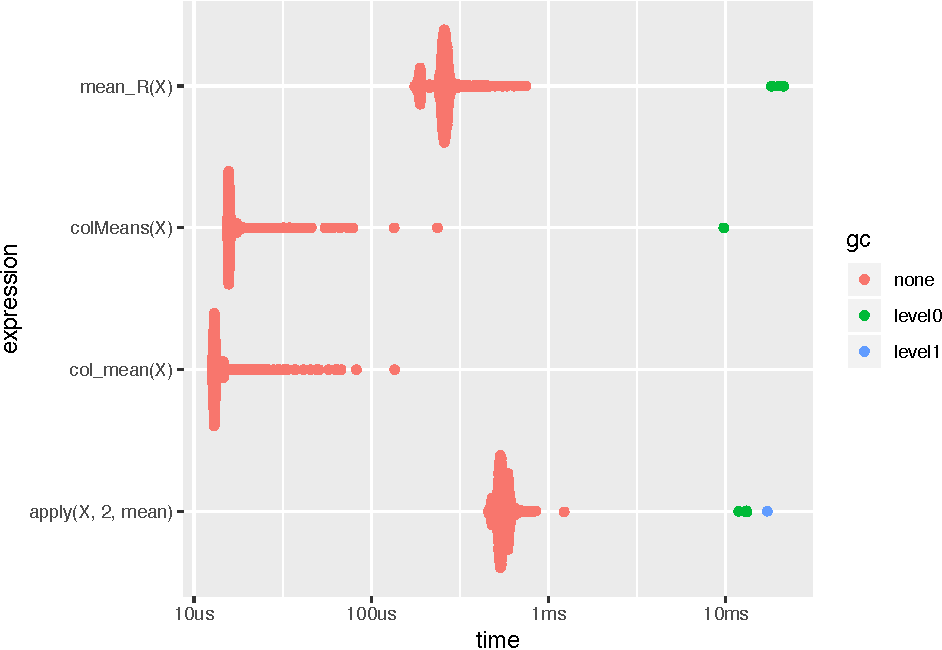
\includegraphics{bookdown_files/figure-latex/unnamed-chunk-40-1.pdf}

对比结果如图所示,其中gc\footnote{垃圾回收(英语:Garbage Collection,缩写为GC),在计算机科学中是一种自动的存储器管理机制。当一个计算机上的动态存储器不再需要时,就应该予以释放,以让出存储器,这种存储器资源管理,称为垃圾回收。}是一个关于内存使用的指标,越低越好.

apply和在R中用循环编写函数速度差不多,用C++编写的函数明显比其他快,甚至比base库中的函数还要快.不过,当我们增加矩阵的大小时,就会发现不一样的结果:

\begin{Shaded}
\begin{Highlighting}[]
\NormalTok{Rcpp}\OperatorTok{::}\KeywordTok{sourceCpp}\NormalTok{(}\StringTok{'code/Rcpp-demo.cpp'}\NormalTok{)}
\end{Highlighting}
\end{Shaded}

\begin{verbatim}
## 
## > mean_R <- function(X) {
## +     n = dim(X)[1]
## +     m = dim(X)[2]
## +     cm <- rep(0, m)
## +     for (i in 1:n) {
## +         cm = cm + X[i, ]
## +     }
## +    .... [TRUNCATED]
\end{verbatim}

\begin{Shaded}
\begin{Highlighting}[]
\NormalTok{m =}\StringTok{ }\DecValTok{2000}
\NormalTok{n =}\StringTok{ }\DecValTok{1000}
\NormalTok{X <-}\StringTok{ }\KeywordTok{matrix}\NormalTok{(}\KeywordTok{rnorm}\NormalTok{(m}\OperatorTok{*}\NormalTok{n),m,n)}
\KeywordTok{col_mean}\NormalTok{(X) ->}\StringTok{ }\NormalTok{l1}
\KeywordTok{mean_R}\NormalTok{(X) ->}\StringTok{ }\NormalTok{l2}
\KeywordTok{all.equal}\NormalTok{(l1,l2)}
\end{Highlighting}
\end{Shaded}

\begin{verbatim}
## [1] TRUE
\end{verbatim}

\begin{Shaded}
\begin{Highlighting}[]
\KeywordTok{colMeans}\NormalTok{(X) ->}\StringTok{ }\NormalTok{l3}
\KeywordTok{all.equal}\NormalTok{(l1,l3)}
\end{Highlighting}
\end{Shaded}

\begin{verbatim}
## [1] TRUE
\end{verbatim}

\begin{Shaded}
\begin{Highlighting}[]
\KeywordTok{apply}\NormalTok{(X, }\DecValTok{2}\NormalTok{, mean) ->}\StringTok{ }\NormalTok{l4}
\KeywordTok{all.equal}\NormalTok{(l1,l4)}
\end{Highlighting}
\end{Shaded}

\begin{verbatim}
## [1] TRUE
\end{verbatim}

\begin{Shaded}
\begin{Highlighting}[]
\NormalTok{bench}\OperatorTok{::}\KeywordTok{mark}\NormalTok{(}
  \KeywordTok{col_mean}\NormalTok{(X),}
  \KeywordTok{colMeans}\NormalTok{(X),}
  \KeywordTok{mean_R}\NormalTok{(X),}
  \KeywordTok{apply}\NormalTok{(X, }\DecValTok{2}\NormalTok{, mean),}
  \DataTypeTok{check =} \OtherTok{FALSE}\NormalTok{,}\DataTypeTok{relative =} \OtherTok{TRUE}
\NormalTok{)->results}
\NormalTok{ggplot2}\OperatorTok{::}\KeywordTok{autoplot}\NormalTok{(results)}
\end{Highlighting}
\end{Shaded}

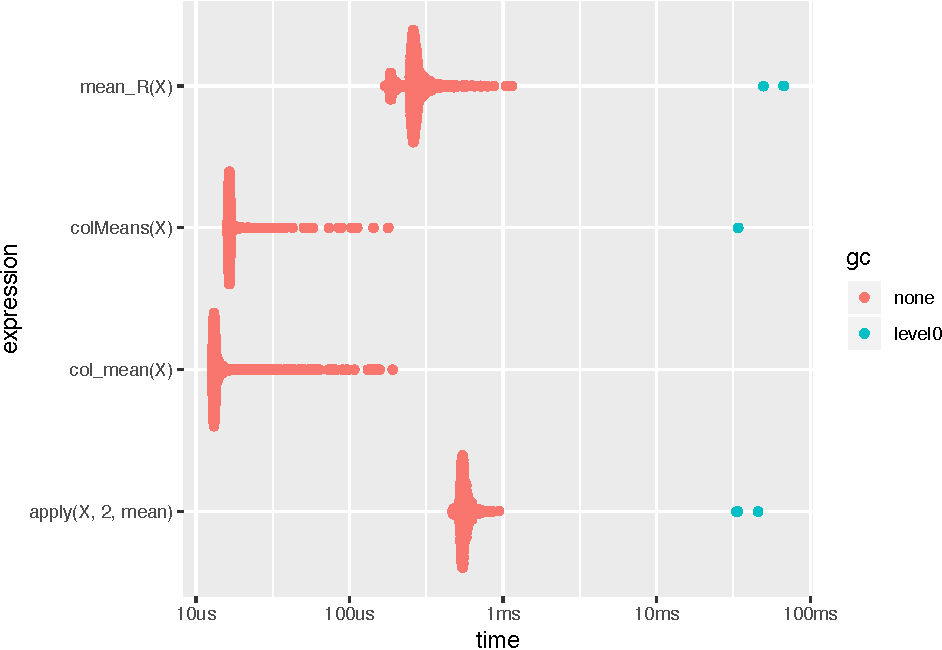
\includegraphics{bookdown_files/figure-latex/unnamed-chunk-41-1.pdf}

可以看到,还是base库中提供的函数速度最快.

\hypertarget{rcppparallel}{%
\subsection{RcppParallel}\label{rcppparallel}}

C++并行库

\href{https://rcppcore.github.io/RcppParallel/index.html}{官方文档}

这里提供一个RcppParallel的例子:
\href{https://github.com/Ri0016/kernelCpp}{核估计}

下面是三个关于线性代数的库,\url{https://gist.github.com/wolfv/ca3ac2b24e1daf70f85eac18ec7b1b8f}
这个例子的测试结果表明xtensor最快

\hypertarget{rcpparmadillo}{%
\subsection{RcppArmadillo}\label{rcpparmadillo}}

线性代数库
\href{https://cran.r-project.org/web/packages/RcppArmadillo/RcppArmadillo.pdf}{官方文档}

\hypertarget{rcppeigen}{%
\subsection{RcppEigen}\label{rcppeigen}}

线性代数库(更快一点,但是不友好)
\href{https://cran.r-project.org/web/packages/RcppEigen/RcppEigen.pdf}{官方文档}

\hypertarget{xtensor}{%
\subsection{xtensor}\label{xtensor}}

\href{https://github.com/QuantStack/xtensor-r}{GitHub地址}

\cleardoublepage

\hypertarget{appendix-}{%
\appendix \addcontentsline{toc}{chapter}{\appendixname}}


\hypertarget{sound}{%
\chapter{余音绕梁}\label{sound}}

呐,到这里朕的书差不多写完了,但还有几句话要交待,所以开个附录,再啰嗦几句,各位客官稍安勿躁、扶稳坐好。

\bibliography{book.bib,packages.bib}

\backmatter
\printindex

\end{document}
